\documentclass[10pt,a4paper]{article}
\usepackage[T1]{fontenc}
\usepackage[scaled]{helvet}
\usepackage{cite}
\usepackage{url}
\usepackage{graphicx}
\usepackage{listings}
\usepackage{float}
\usepackage{amsmath}
\usepackage{amssymb}
\usepackage{fancyhdr}
\usepackage{lastpage}
\floatstyle{boxed} 
\restylefloat{figure}
\renewcommand*\familydefault{\sfdefault}
\title{Process Management and IPC}
\author{David Lynch - david.lynch@raglansoftware.com }
\begin{document}
\maketitle
\begin{abstract}
This article will dig into the details of process management and inter-process communication(IPC). It is important for any programmer to understand the process lifecycle, and in particular to ensure that any applications that are written correctly leverage these functions, in particular provider clear entry and exit points. When modularizing function into separate components, how these processes communicate also becomes a very important tool in the armoury.
\end{abstract}
\section{Process Management}
A {\bf process} is an active entity of work in a computer system. A process will consist of some code, or more formally a text-section. There are a number of things that the operating system will store that are associated with each process. Firstly, a copy of the {\bf program counter} and {\bf CPU} register file is necessarily kept. When the process is context switched, in order to resume from the exact location we left off, we must restore these. Another important entity associated with a process is its stack. This can be thought of as a region of memory that contains state that is typically local to the function or method that is currently executing. Function parameters, local variables and return variables are all kept on the stack, and this stack will typically be multiple layers deep. The depth depends on how many seperate function calls have not yet returned in any particular process. Separate to the process stack we have {\bf heap memory}. This memory is a region that is usable by a process, but is dynamically allocated at runtime by the application and the operating system.
\subsection{State}
Speaking generally, a process can be any number of five states. Different operating systems will have different states, usually reflecting things like priority, but each can be distilled as follows. 
\begin{itemize}
\item New - The Process is undergoing creation.
\item Running - Instructions are being executed.
\item Waiting - The process is stalled waiting for some event.
\item Terminated - The process has finished execution.
\end{itemize}
On process may run on one processor at any one time, while many processes can be in the ready and weating states. 
\begin{figure}
\caption{The Process State Life-Cycle \cite{OSCONCEPTS}}
\begin{center}
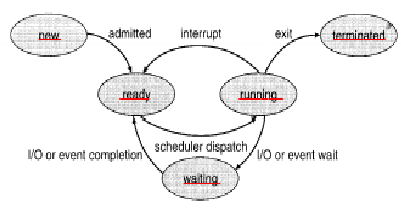
\includegraphics[scale=0.45]{../images/process-state.png}
\label{procstate}
\end{center}
\end{figure}
\subsection{Process Control Block}
Frequently referred to as the PCB, the process control block is an explicit collection of all the important data that surrounds the management of a process. The following data is part of the process control block. Code examples show how the Linux kernel implements each of these. 
\subsubsection{Process State} 
This indicator maintains the state of the process and gets updated as the process transitions between states. 
\begin{lstlisting}
put your code here
\end{lstlisting}
\subsubsection{Program Counter}
The address register that points to the next instruction that should be executed in the process. 
\subsubsection{Register State}
The internal register state includes information, such as partial results of programs, and stack pointers.
\subsubsection{CPU Schedule Information}
The most common piece of information here is the priority of the process. Some more complex information may also be recorded here, in particular how long the process has been running, and or how long the process has be in it's current state without gaining control of the CPU.  
\subsubsection{Memory Management Information}
Memory information is associated with this section includes the contents of segment registers, or page tables. This information assists in mapping memory locations on the heap with the process. Also, virtual memory page tables are maintained for the parts of the process that have not yet been loaded to disk. 
\subsubsection{Accounting Information}
The ID of the process, which CPU is been used and for how long and some limits on the quota of these is all considered accounting information usually associated with a process. 
\subsubsection{I/O Status Information}
This information relates to files that may be open by the process. 
\section{Process Scheduling}
The objective of {\bf multi-programming} is to have some process executing on the CPU at all times. The {\bf process scheduler} selects an available process based on some criteria. The {\bf job queue} consists of all processes in the system. This is a broader view of the whole system, but for practical purposes this is broken down into several queues, typically associated with the state of the process. Processes in memory and ready to execute are placed in the {\bf ready queue}.  Processes waiting on a particular I/O device are on the {\bf device queue}. When a process is selected for execution it is {\bf dispatched} by an operating system component known as the {\bf dispatcher}. Once a process is dispatched it can issue an I/O request and get placed on the device queue, create a new sub-process and wait around for it's termination, execute some instructions on its own data or be forcibly removed from the CPU to the ready queue as the result of an interrupt. 
\subsection{Schedulers}
A process will move between various queues over its lifetime. This is managed by a number of schedulers. The {\bf process scheduler} selects a process from a pool of candidates and loads them into memory for execution. The {\bf CPU scheduler} selects processes from memory and allocates access to the CPU for a period of time. Each scheduler will implement one or more algorithms, each of which is chosen based on a set of desired criteria. The simplest objective for a process scheduler is to aim to ensure a good balance between {\bf I/O bound} and {\bf CPU bound} processes. At the CPU level, the priority is typically to maximize the utilization of the CPU. 
\subsection{Context Switch}
When an interrupt causes the operating system to change the currently executing task to some other task it is necessary to execute some management tasks. In essence, the current {\bf context} is defined by the contents of the process control block. When the process control block is written and saved, either to backing store or memory, it is known as a context switch. Context switching is totally overhead and a very important cost to consider in a multi-programming environment. This cost is comprised of memory write cycles, and possibly disk write cycles to save the state of the process control block. However, emptying of the CPU pipeline and likely invalidation of multiple levels of CPU cache must also be factored into this cost. 
\subsection{Process Creation}
A {\bf tree of processes} is created by a some process creating a child process and, in turn, that child process creating further children. Upon creation of a process, it is assigned a unique {\bf process identifier}. Sub-processes can be restricted to a subset of the parents resources and can also share state and resources with its parent. A parent process may execute {\bf concurrently} with its children, or it may hang around and wait for its children to terminate before exiting. A child process typically duplicates the parents' process, sharing its address space. 
\newline\newline
\subsubsection{Examples}
In Linux the {\it fork} system call will create the new process. After this call is invoked both processes continue execution. The return type of the fork call is an it integer, which will be used within the program to understand which process is currently executing. If this value is zero, we are currently in the child process. Figure \cite{fork} illustrates an example. The {\it exclp} system call will replace the currently executing process image with a new image. In this case, the forked child process executes the Linux {\it ls} command which will list the files in the current directory. The parent process simply waits until the forked child completes and exits. 
\newline\newline
Type out the sample program listing here.  
\newline\newline
The analogous system call on Windows is \{it CreateProcess}. It is pretty much similar in all respects except that it requires the loading of a specified program into the address space of the child process, whereas this is not explicitly required with fork. 
\newline\newline
Type out the sample windows program listing here. 
\subsection{Process Termination}
A program will execute when it execute its last statement and invokes the {\it exit} system call. At this point a process may return some value to its parent. All resources allocated to the process are de-allocated by the operation system, although typically the safe de-allocation of resources is only guaranteed when the process is typically executed. A child may be terminated if it has exceeded its usage of resources, if the task is no longer required and killed by a user or if it's parent process is terminating. 
\section{Inter-Process Communication}
Processes being executed concurrently by the OS may be either {\bf independent} or {\bf co-operating}. There are a number of advantages to processes co-operating to get a specific set of work done. Files, or other data may be shared between processes. This is particularly useful if retrieving the data in the first instance is an expensive operation. Breaking processes into sub-process can assist in speed of execution, particularly if the executing program lends itself to parallelism. For example, a web-crawler process that is responsible for downloading and parsing web-pages could share the same program text, but differ in the URL as a parameter. Retrieving a web-page is an I/O intensive operation, which involves some waiting, so even at the CPU level there is some benefit to have two of the same processes waiting on I/O from two different requests in parallel.  Another benefit is modularity of design, which facilitates simplicity of understanding and development for the programmer. However, in order to accomplish this communication, the operating system must facilitate the programmer via a system call. 
\subsection{Shared Memory}
In this method, process that wish to communicate establish a region of shared memory that resides in the address space of the initializing process. Other processes wishing to communicate will attach to this address space. This requires the process to circumvent the OS restriction that processes cannot reference the address space of other processes. Therefore the operating system must facilitate this interaction by means of system call. The Linux system call that facilitates this is {\it shmget}. A good use case for shared memory is where a producer/consumer relationship exists between the processes. A simple bounded, or unbounded, buffer is constructed between the two processes using a shared memory space. 
\subsection{Message Passing}
In order to avoid sharing an explicit memory address space, a process can leverage message passing. This facilitates processes in synchronizing their actions without allocating a shared location in memory. This is particularly useful in the cases where sharing of an address spaces is not possible, such as when processes are located on different machines. There are two operations, {\it send(message)} and {\it receive(message)}. Message structure and size can be defined by the processes that are communicating, but can vary depending on implementation. In order for processes to communicate at least a logical communication link must exist between the processes. 
\subsubsection{Direct or Indirect}
For direct communication, processes much know each others identity. This is known as symmetric addressing.  Exactly one link can then be established between a pair of processes, with a single link associated with exactly two processes. Conversely, for indirect or asymmetric addressing, the receive end of the communication pair does not need to know the identity of the link from which it is accepting a message. To facilitate this, messages are sent to {\bf ports} or {\bf mailboxes}. The link between processes is only established if they actually share a mailbox. In the case of indirect communication, a link may be associated with more than two processes and multiple links may exist between two processes.
\subsection{Synchronization} 
\subsubsection{Synchronous or Asynchronous}
\subsubsection{Buffering}


\subsection{Message Passing}

\bibliography{../biblio/techfundamentals.bib}{}
\bibliographystyle{plain}
\begin{center}
{\small \copyright  David Lynch 2012. Do not reproduce without written permission.}
\end{center}
\end{document}
